\documentclass[a4paper,oneside,DIV=10,12pt]{scrartcl}

\usepackage{float}

\usepackage{fontspec}
\setmainfont{PT Serif}
\setsansfont{PT Sans}
\setmonofont{PT Mono}

\usepackage{microtype}

\usepackage{amsmath}
\usepackage{unicode-math}
\setmathfont{STIX Two Math}

\usepackage{polyglossia}
\setmainlanguage{russian}

\usepackage{graphicx}

\usepackage{listings}

\usepackage{siunitx}

\usepackage{hyperref}

\newcommand\filename[1]{\texttt{#1}}
\newcommand\modulename[1]{\texttt{#1}}

\newfloat{lstfloat}{htbp}{lop}
\floatname{lstfloat}{Листинг}

\begin{document}
	\lstset{
		basicstyle=\ttfamily,
		breaklines=true,
	}
	
	\title{Как пользоваться скриптом для построения графиков для лаб по электронике}
	\date{}
	\author{}
	
	\maketitle
	
	\tableofcontents
	
	\section{Что это?}
	
	Это руководство пользователя скрипта, который строит графики для лаб по электронике. Он работает, считывая данные файла, сгенерированного графопостроителем Воркбенча, и по его содержанию строит нужные графики. То есть по такой цепочке:
	\begin{enumerate}
		\item Воркбенч
		\item Файл с координатами графиков
		\item Скрипт
		\item Графики
	\end{enumerate}
	
	\section{Перед работой}
	Для правильной работы скрипта необходимы:
	\begin{enumerate}
		\item Рабочий Electronics Workbench (тут использовалась версия 5.12).
		\item Рабочий Python 3 с поддержкой Tk (если во время установки Python вы нажали «Install Now», он у вас есть).
		\item Два установленных модуля для Python:
			\begin{enumerate}
				\item \modulename{matplotlib}
				\item \modulename{numpy}
			\end{enumerate}
	\end{enumerate}
	
	Если Python не установлен, его надо скачать и установить с официального сайта (\url{https://www.python.org/ftp/python/3.6.3/python-3.6.3.exe}). При установке установить галочку «Add Python 3.6 to PATH» и нажать кнопку «Install Now».
	
	Желательно иметь Python в \verb|%PATH%|, чтобы обращаться к нему прямо, не указывая полного пути к интерпретатору. Чтобы проверить, есть ли Python в \verb|%PATH%|, достаточно в командной строке ввести команду из листинга \ref{checkpython}.
	
		\begin{lstfloat}
		\begin{lstlisting}
python --version
		\end{lstlisting}
		\caption{Команда для проверки наличия Python}
		\label{checkpython}
	\end{lstfloat}
	
	Если Python установлен и указан в переменной среды \verb|%PATH%|, вывод будет примерно таким:
	
	\begin{verbatim}Python 3.5.1\end{verbatim}
	
	Так как \modulename{matplotlib} и \modulename{numpy} не идут в комплекте стандартной поставки Python, их надо установить. Для этого в командной строке запустим команду из листинга \ref{installmodules}.
	
	\begin{lstfloat}
		\begin{lstlisting}
pip install matplotlib numpy
		\end{lstlisting}
		\caption{Команда для установки необходимых модулей}
		\label{installmodules}
	\end{lstfloat}
	
	Если модули установились успешно и все остальные необходимые составляющие на месте, скрипт готов к работе.
	
	\section{Как пользоваться?}
		\subsection{Получение файла с координатами}
		Для начала необходимо получить файл с координатами графиков. Для этого в Воркбенче открываем лабу и выполняем всё по тексту лабы до тех пор, пока на осцилографе не будет показана нужная осцилограмма (рис. \ref{fig:oscilloscope}).
	
		\begin{figure}[H]
			\centering
			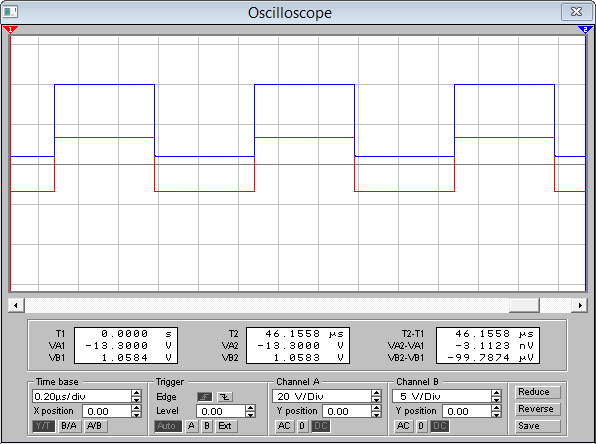
\includegraphics[width=\textwidth]{step01.png}
			\caption{На экране осцилографа появилась осцилограмма}
			\label{fig:oscilloscope} 
		\end{figure}
	
		Скрипту не важны никакие настройки масштаба (Time base, Channel A и Channel B) и положение визирных линий, так как он работает непосредственно с получеными данными. Главное, чтобы был правильно выставлен режим работы (Y/T, Auto, DC, DC) и сама схема была настроена так, как описано в тексте лабы.
		
		Далее, чтобы получить файл с координатами, открываем графопостроитель и с его помощью экспортируем файл. Для этого нажимаем на кнопку «Display Graphs» (тулбар в главном окне, пиктограмма с двумя графиками). На экране откроется окно графопостроителя (рис. \ref{fig:grapher}).
		
		\begin{figure}[H]
			\centering
			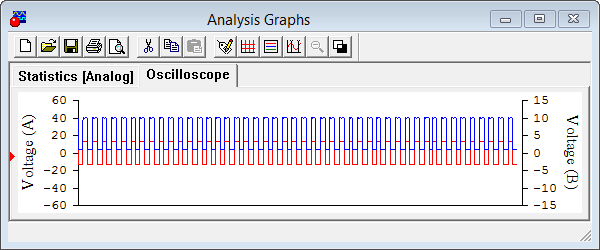
\includegraphics[width=\textwidth]{step02-1.png}
			\caption{Окно графопостроителя}
			\label{fig:grapher} 
		\end{figure}
		
		Затем, в окне графопостроителя, нажимаем на кнопку «Save As» (дискета), и сохраняем файл в удобном месте (рис. \ref{fig:saving}). Желательно, в той же папке, что и сам скрипт. \emph{Внимание!} Очень важно, чтобы тип файла был именно «Graph Data (.txt)», потому что скрипт писался для обработки именно этого типа файла.
		
		\begin{figure}[H]
			\centering
			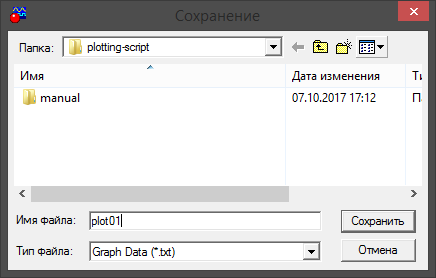
\includegraphics[]{step03.png}
			\caption{Параметры сохранения}
			\label{fig:saving} 
		\end{figure}
		
		После сохранения в выбранной папке появится текстовый файл (в данном случае, \filename{plot01.txt}). Именно этот файл нужен для построения графиков с помощью скрипта.
		
		\subsection{Построение графиков скриптом}
		Теперь необходимо передать полученный файл скрипту на обработку. Для этого открываем коммандную строку и переходим в папку, которая содержит сам скрипт и файл с графиком. Затем, выполняем комманду с рис. \ref{fig:cmd}.
		
		\begin{figure}[H]
			\centering
			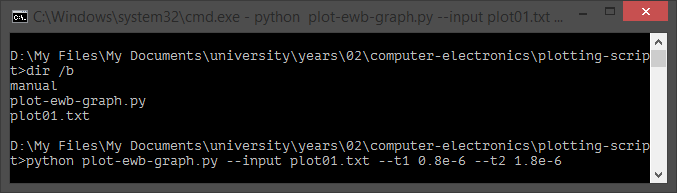
\includegraphics[width=\textwidth]{step04-1.png}
			\caption{Запуск скрипта}
			\label{fig:cmd} 
		\end{figure}
		
		После запуска скрипта должно появиться окно с построенными графиками (рис. \ref{fig:plots}).
		
		\begin{figure}[H]
			\centering
			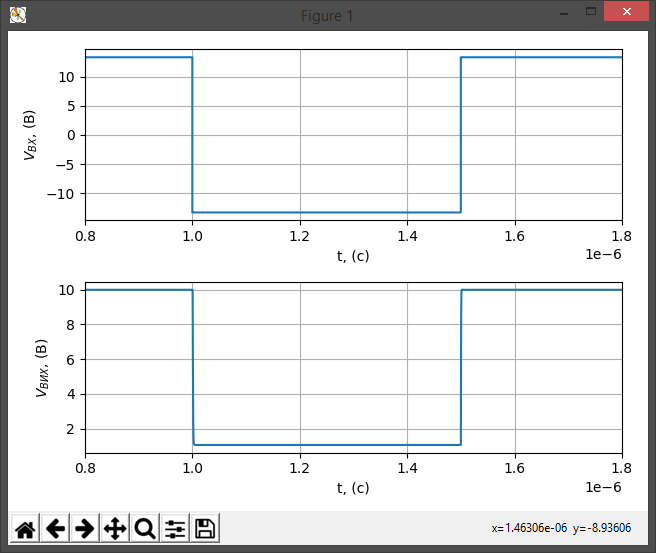
\includegraphics[width=0.8\textwidth]{step05.png}
			\caption{Окно с построенными графиками}
			\label{fig:plots} 
		\end{figure}
		
		Cкрипт запускается командой по типу листинга \ref{runscript}. Интерпретатор Python на Windows почему-то не хочет сразу подхватывать скрипт, поэтому скрипт необходимо запускать, указывая имя интерпретатора перед именем скрипта.
		
		\begin{lstfloat}
			\begin{lstlisting}
python plot-ewb-graph.py --input plot01.txt --t1 0.8e-6 --t2 1.8e-6
			\end{lstlisting}
			\caption{Пример команды для построения графиков скриптом}
			\label{runscript}
		\end{lstfloat}
		
		Рассмотрим параметры, которые были указаны, чтобы получить графики с рис. \ref{fig:plots}:
		\begin{enumerate}
			\item \lstinline!python plot-ewb-graph.py! --- запуск скрипта.
		
			\item \lstinline!--input plot01.txt! --- в качестве входного файла использовать \filename{plot01.txt}.
		
			\item \lstinline!--t1 0.8e-6 --t2 1.8e-6! --- построить графики для временного промежутка от $t_1 = \SI{0.8e-6}{\second}$ до $t_2 = \SI{1.8e-6}{\second}$.
		\end{enumerate}
		
		Временные параметры нужно выбирать так, чтобы график показывал как минимум один полупериод, то есть чтобы потом было удобно показать $t_{\text{ЗД}}, t_{\text{НР}}, t_{\text{Р}}, t_{\text{СП}}$. Если вдруг параметры были выбраны неправильно, можно нажать на кнопку с четырьмя стрелочками и подвигать любой из графиков. Таким образом можно узнать удобный временной промежуток и перезапустить скрипт с новыми параметрами.
		
		\subsection{Сохранение построенных графиков}
		Для сохранения графиков достаточно в окне с построенными графиками нажать на кнопку «Save the figure». При сохранении можно выбрать любой удобный формат: JPEG, PNG, SVG и т.д. Советую сохранять в векторном формате (SVG), чтобы график можно было масштабировать без потерь и сжатия.
	
	\section{Примечания}
		Чтобы строить графики с другими настройками электрической схемы, наверное, удобнее всего будет каждый раз закрывать лабу, выставлять нужные настройки, строить осцилограмму по новой и сохранять в отдельный файл. Это делается для того, чтобы не запутаться в том, какая диаграмма для каких настроек.
		
		Допустим, открыли лабу и настроили на напряжение \SI{10}{\volt} без подключенного диода. Построили осцилограмму, получили файл, назвали его \filename{1.5v\-no\-diode.txt}, построили график, экспортировали его. Потом закрыли лабу и настроили на то же напряжение, но теперь \emph{с диодом}. Построили осцилограмму, получили файл, назвали его \filename{1.5v-diode.txt}, построили график, экспортировали его. И так для каждого нужного значения.
		
		На полученных диаграммах нужно обозначить $t_{\text{ЗД}}, t_{\text{НР}}, t_{\text{Р}}, t_{\text{СП}}$ по примеру с рис. \ref{fig:timediag} (взят из методички). 
		
		\begin{figure}[H]
			\centering
			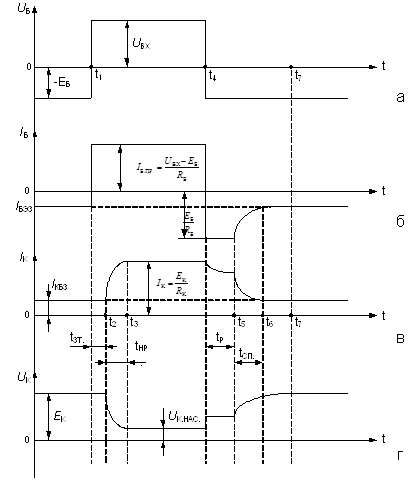
\includegraphics[]{timediag.png}
			\label{fig:timediag} 
		\end{figure}
		
		Единицы измерения временной оси $OX$ — секунда, но на графике отмечены значения 0.8, 1.0, 1.2 и т.д. Это не секунды, а \emph{микросекунды}. Дело в том, что на оси стоит обозначение 1e−6, что означает, что любое обозначенное значение на оси $OX$ мы должны умножить на \num{1e-6}. Таким образом получаем микросекунды. Иначе говоря, что бы там препод не говорил, масштаб правильный, просто надо уметь читать обозначения. Или можно в любом редакторе закрасить 1e−6, а на оси изменить t, (с) на t, (мкс).
		
		Как и во всех нормальных графиках, на координатных осях нет стрелочек. Направление оси очевидно по значениям. Возможно, преподу это не понравится — можно дорисовать.
\end{document}